% Extracted from maximumsAndMinimums.tex, problem #2
\begin{problem}
	The entire graph of a function $g$ is given below.
				\begin{center}
					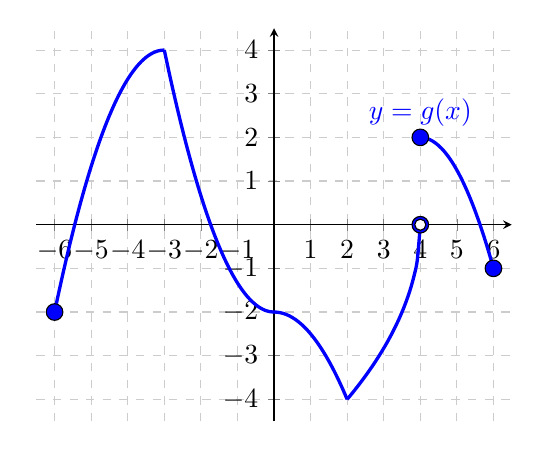
\begin{tikzpicture}
						\begin{axis}[
							xmin=-6.5, xmax=6.5, ymin=-4.5,ymax=4.5,    
							axis lines =middle, 
							every axis y label/.style={at=(current axis.above origin),anchor=south},
							every axis x label/.style={at=(current axis.right of origin),anchor=west},
							xtick={-6,...,6}, ytick={-4,...,4},
							grid=major, width=3in,
							grid style={dashed, gray!40} 
							]
							\addplot[color=blue, very thick, smooth, domain=-6:-3]{-(2/3)*(x+3)^2+4};
							\draw[fill=blue] (axis cs:-6,-2) circle [color=blue,radius=3pt] node [below right] {};						
						
							\addplot[color=blue, very thick, smooth, domain=-3:0]{(2/3)*x^2-2};						
							\addplot[color=blue, very thick, smooth, domain=0:2]{-(1/2)*x^2-2};												
							\addplot[color=blue, very thick, smooth, domain=2:4]{-(8^(0.5))*(4-x)^(0.5)};																		
							\addplot[color=blue, very thick, smooth, domain=4:6]{-(3/4)*(x-4)^2+2} node[anchor=south,pos=0]{$\Large{y=g(x)}$};
							
							\draw[fill=blue] (axis cs:6,-1) circle [color=blue,radius=3pt] node [below right] {};						
							\draw[fill=blue] (axis cs:4,2) circle [color=blue,radius=3pt] node [below right] {}; 					
													
						\draw[fill=blue] (axis cs:4,0) circle [color=blue,radius=3pt] node [below right] {};
						\draw[fill=white] (axis cs:4,0) circle [color=white,radius=2pt] node [below right] {};
						
						
						
						\end{axis}
					\end{tikzpicture}
				\end{center}
	Based on the graph of $g$, answer the questions below.
	\begin{enumerate}
		\item List the $x$-coordinates of all critical points of $g$.
\WkstHop
			\begin{freeResponse}
				$x = -3$, $x=0$, $x=2$, and $x=4$.
			\end{freeResponse}
		\item List the $x$-coordinates of all critical points of $g$ where $g'(x)=0$.
\WkstHop
			\begin{freeResponse}
				$x = 0$
			\end{freeResponse}
		\item List the $x$-coordinates of all critical points of $g$ where $g'(x)$ is \textbf{undefined}.
\WkstHop
			\begin{freeResponse}
				$x = -3$, $x=2$, and $x=4$.
			\end{freeResponse}
		\item List the $x$-coordinates of all local maximums of $g$.
\WkstHop
			\begin{freeResponse}
				$x = -3$ and $x=4$.
			\end{freeResponse}
		\item List the $x$-coordinates of all local minimums of $g$.
\WkstHop
			\begin{freeResponse}
				$x=2$
			\end{freeResponse}		
		\item List all intervals where $g$ is both decreasing AND concave down.
\WkstHop
			\begin{freeResponse}
				$(0,2)$ and $(4,6)$.
			\end{freeResponse}			
		\item List all intervals where $g$ is both decreasing AND concave up.
\WkstHop
			\begin{freeResponse}
				$(-3,0)$ 
			\end{freeResponse}
		\item List all intervals where $g$ is both increasing AND concave down.
\WkstHop
			\begin{freeResponse}
				$(-6,-3)$
			\end{freeResponse}		
		\item List all intervals where $g$ is both increasing AND concave up.
\WkstHop
			\begin{freeResponse}
				$(2,4)$
			\end{freeResponse}		
		\item List the $x$-coordinates of all inflection points of $g$.
\WkstHop
			\begin{freeResponse}
				$x=-3$, $x=0$, and $x=2$.
			\end{freeResponse}		
	\end{enumerate}
\end{problem}
